%%%%%%%%%%%%%%%%%%%%%%%%%%%%%%%%%%%%%%%%%%%%%%%%%%%%%%%%%%%%%%%%%%%%%%%%%%%%%%%%%%%%%%%%%%%%%%%%%%%%%%%
%%%%%%%%%%%%%% Template de Artigo Adaptado para Trabalho de Diplomação do ICEI %%%%%%%%%%%%%%%%%%%%%%%%
%% codificação UTF-8 - Abntex - Latex -  							     %%
%% Autor:    Fábio Leandro Rodrigues Cordeiro  (fabioleandro@pucminas.br)                            %% 
%% Co-autor: Prof. João Paulo Domingos Silva, Harison da Silva e Anderson Carvalho                   %%
%% Revisores normas NBR (Padrão PUC Minas): Helenice Rego Cunha e Prof. Theldo Cruz                  %%
%% Versão: 1.1     18 de dezembro 2015                     	                                     %%
%%%%%%%%%%%%%%%%%%%%%%%%%%%%%%%%%%%%%%%%%%%%%%%%%%%%%%%%%%%%%%%%%%%%%%%%%%%%%%%%%%%%%%%%%%%%%%%%%%%%%%%


\documentclass[a4paper,12pt,Times]{article}
\usepackage{abakos}  %pacote com padrão da Abakos baseado no padrão da PUC

%%%%%%%%%%%%%%%%%%%%%%%%%%%
%Capa da revista
%%%%%%%%%%%%%%%%%%%%%%%%%%

%\setcounter{page}{80} %iniciar contador de pagina de valor especificado
\newcommand{\monog}{Artigo sobre Dispositivos Lógicos Programáveis}
\newcommand{\monogES}{Article about Programmable Logic Devices}
\newcommand{\tipo}{Artigo }  % Especificar a seção tipo do trabalho: Artigo, Resumo, Tese, Dociê etc
\newcommand{\origem}{Brasil }
\newcommand{\editorial}{Belo Horizonte, p. 01-7, mar. 2022}   % p. xx-xx – páginas inicial-final do artigo
\newcommand{\lcc}{\scriptsize{Licença Creative Commons Attribution-NonCommercial-NoDerivs 3.0 Unported}}

%%%%%%%%%%%%%%%%%INFORMAÇÕES SOBRE AUTOR PRINCIPAL %%%%%%%%%%%%%%%%%%%%%%%%%%%%%%%
\newcommand{\AutorA}{Julia Veloso Dias}
\newcommand{\funcaoA}{}
\newcommand{\emailA}{julia.dias@pucminas.br}
\newcommand{\cursA}{Aluno do Programa de Graduação em Ciência da Computação}
% 
% Definir macros para o nome da Instituição, da Faculdade, etc.
\newcommand{\univ}{Pontifícia Universidade Católica de Minas Gerais}

\newcommand{\keyword}[1]{\textsf{#1}}

\begin{document}
% %%%%%%%%%%%%%%%%%%%%%%%%%%%%%%%%%%
% %% Pagina de titulo
% %%%%%%%%%%%%%%%%%%%%%%%%%%%%%%%%%%

\begin{center}

\includegraphics[scale=0.2]{figuras/brasao.jpg} \\
PONTIFÍCIA UNIVERSIDADE CATÓLICA DE MINAS GERAIS \\
Instituto de Ciências Exatas e de Informática

% \vspace{1.0cm}

\end{center}

 


\vspace{1.0cm}

\begin{flushright}
\singlespacing 
\normalsize{\AutorA \footnote{\funcaoA \cursA, \origem -- \emailA . }} 


\end{flushright}
\thispagestyle{empty}

\vspace{1.0cm}

\begin{abstract}
\noindent
O principal objetivo que hoje a computação busca é o melhor desempenho em seus programas e assim como todos os métodos computacionais, os PLDs (Programmable Logic Device) que tem sua funcionalidade para automação industrial, visam encontrar o menor custo para grandes produções e por isso é interessante aplicar a lógica programável nesse contexto, essa qual permite que qualquer circuito binacional seja descrito em uma soma com vários mintermos, estes os produtos entre as variáveis da tabela-verdade.
O artigo procura explicar todos os termos que foram direcionados para identificação no enunciado da atividade prática, estes baseados na soma de produtos (SDP), baseado em outros artigos propostos além de um que está a escolha do aluno. 
\\\textbf{\keyword{Palavras-chave: }} Dispositivos Lógicos Programavéis.
\end{abstract}

%%%%%%%%%%%%%%%%%%%%%%%%%%%%%%%%%%%%%%%%%%%%%%%%%%%%%%%%%
 \newpage    %%%% CASO QUEIRA QUE O RESUMO FIQUE EM UMA PAGINA E O ABSTRACT EM OUTRA
\selectlanguage{english}
\begin{abstract}
\noindent
The main objective that computing today seeks is the best performance in its programs and, like all computational methods, PLDs (Programmable Logic Device) that have their functionality for industrial automation, aim to find the lowest cost for large productions and that is why it is It is interesting to apply programmable logic in this context, which allows any binational circuit to be described in a sum with several minterms, these being the products between the variables of the truth table.
The article seeks to explain all the terms that were directed to identification in the practical activity statement, these based on the sum of products (SDP), based on other proposed articles in addition to one that is the student's choice.
\\\textbf{\keyword{Keywords: }} Programmable Logic Devices.
\end{abstract}

\selectlanguage{brazilian}
 \onehalfspace  % espaçamento 1.5 entre linhas
 \setlength{\parindent}{1.25cm}

%%%%%%%%%%%%%%%%%%%%%%%%%%%%%%%%%%%%%%%%%%%%%%%%%
%% INICIO DO TEXTO
%%%%%%%%%%%%%%%%%%%%%%%%%%%%%%%%%%%%%%%%%%%%%%%%%

%%%%%%%%%%%%%%%%%%%%%%%%%%%%%%%%%%%%%%%%%%%%%%%%%%%%%%%%%%%%%%%%%%%%%%%%%%%%%%%%%%%%%%%%%%%%%%%%%%%%%%%
%%%%%%%%%%%%%% Template de Artigo Adaptado para Trabalho de Diplomação do ICEI %%%%%%%%%%%%%%%%%%%%%%%%
%% codificação UTF-8 - Abntex - Latex -  							     %%
%% Autor:    Fábio Leandro Rodrigues Cordeiro  (fabioleandro@pucminas.br)                            %% 
%% Co-autores: Prof. João Paulo Domingos Silva, Harison da Silva e Anderson Carvalho		     %%
%% Revisores normas NBR (Padrão PUC Minas): Helenice Rego Cunha e Prof. Theldo Cruz                  %%
%% Versão: 1.1     18 de dezembro 2015                                                               %%
%%%%%%%%%%%%%%%%%%%%%%%%%%%%%%%%%%%%%%%%%%%%%%%%%%%%%%%%%%%%%%%%%%%%%%%%%%%%%%%%%%%%%%%%%%%%%%%%%%%%%%%
\section{\esp Dispositivos Lógicos Programáveis}

São diversas as tecnologias utilizadas nas construções de circuitos porém os termos que aqui tratados foram antecipadamente especificados e atenderão fielmente ao enunciado proposto.


\subsection{\esp ASICs}

São caratecterizados especialmente por requerir de um processo especial de fabricação, dando a este um alto custo de projeto e longa implementação, quando utilizado em grandes projetos, procura-se fazer uma divisão de testes para tentar melhorar o desempenho.

\subsection{\esp ASSP}

Não foi encontrado o conceito.

\subsection{\esp SPLD}

É um circuto que menos tem custo e possui um desempenho diante os outros. Composto principalmente por portas AND/OR (simples) e pode ter ou não flip-flops na saída.

\subsection{\esp CPLD}

CPLDs são dispositivos programáveis e reprográmaveis pelo usuário, com alto desempenho, baixo custo e alta capacidade de integração.

\subsection{\esp SOC}
Não foi encontrado o conceito.

\subsection{\esp FPGA}

Os FPGAs não possuem planos de port OR/AND, usam na verdade grande arranjo de célula configurável que são implementadas em funções lógicas. Tem como principais recursos: blocos lógicos, blocos de entrada e saída e chaves de interconexão.






\section{\esp Diferenciar}

\subsection{\esp PROM}

São memórias de apenas leitura, porém após a evolução das máquinas, esta permite a programação de usuários.

% Tabela
\begin{table}[htb]
	\centering
	\caption{\hspace{0.1cm} Tabela verdade do decodificador (PROM 8X2)}
	\vspace{-0.3cm} % espaço entre titulo e tabela
	\label{tab:tabela1}
	% Conteúdo da tabela
	\begin{tabular}{l|c |c | c | c}
  \hline
    \textbf{X}	& \textbf{Y} & \textbf{Z}  & \textbf{EXIT 1} & \textbf{EXIT 2} \\
    \hline
        0	& 0 & 0 &  0  &  1  \\
        1	& 0 &  0 & 1 & 1  \\
        0	& 1 & 0 & 1 & 0  \\
        1   &  1 & 0 & 0 & 0  \\
        0	& 0  &  1 & 0 & 1 \\
        1   &  0 & 1 & 0 & 1  \\
        0  & 1  &  1 & 1 & 0 \\
        1  & 1  &  1 & 1 & 1 \\
     \hline
 \end{tabular}
 	\vspace{.1cm}  %espaço entre tabela e fonte
	\small
	% Fonte
	{\footnotesize\\ \textbf{Fonte: “DISPOSITIVOS LÓGICOS PROGRAMÁVEIS”. Profa. Luiza Maria Romeiro Codá. Departamento de Engenharia Elétrica e de Computação.  Acessado em 27/03/2022}}
\end{table}



\subsection{\esp PLA}

Um PLA \textit{(Programmable Logic Array)} um conjunto de arranjos de AND e OR, onde ambos são programáveis e por isso possui um desempenho bom em somo da produtos pois possuem muitas portas.

 \ref{fig:figura1}. 
% Figura
\begin{figure}[ht]
	\centering	
	\caption[\hspace{0.1cm}]{PLA de quatro entradas programadas}
  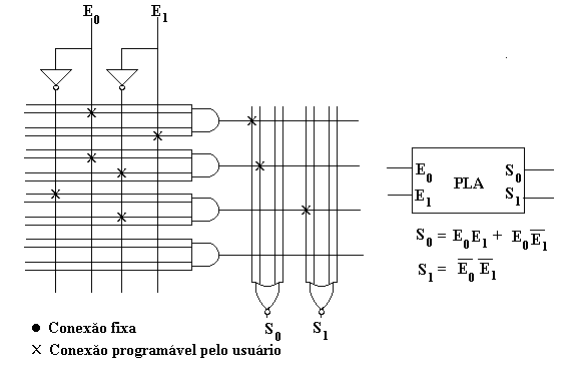
\includegraphics[width=0.4\textwidth]{figuras/pla.png}
	% Caption centralizada
% 	\captionsetup{justification=centering}
	% Caption e fonte 
	 \vspace{-0.2cm}
	\\\textbf{\footnotesize Fonte: Profa. Luiza Maria Romeiro Codá "DISPOSITIVOS LÓGICOS PROGRAMÁVEIS”}
	\label{fig:figura1}
\end{figure}
\vspace{-0.5cm}


\subsection{\esp PAL}

Corresponde a uma matriz lógica programável, é uma forma simplificada da PLA, sendo apenas as portas AND programavél, a matriz OR é fixa.

 \ref{fig:figura1}. 
% Figura
\begin{figure}[ht]
	\centering	
	\caption[\hspace{0.1cm}]{PAL de quatro entradas programadas}
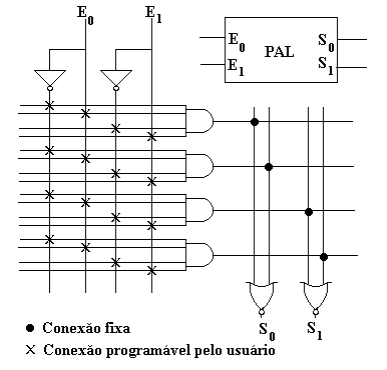
\includegraphics[width=0.4\textwidth]{figuras/PAL.png}
	% Caption centralizada
% 	\captionsetup{justification=centering}
	% Caption e fonte 
	 \vspace{-0.2cm}
	\\\textbf{\footnotesize Fonte: Profa. Luiza Maria Romeiro Codá "DISPOSITIVOS LÓGICOS PROGRAMÁVEIS”}
	\label{fig:figura1}
\end{figure}
\vspace{-0.5cm}


\section{\esp Comparação e diferenciação}

\subsection{\esp CPLD}

São caratecterizados especialmente por requerir de um processo especial de fabricação, dando a este um alto custo de projeto e longa implementação, quando utilizado em grandes projetos, procura-se fazer uma divisão de testes para tentar melhorar o desempenho.

 \ref{fig:figura1}. 
% Figura
\begin{figure}[ht]
	\centering	
	\caption[\hspace{0.1cm}]{Estrutura interna do MAX 7000TM}
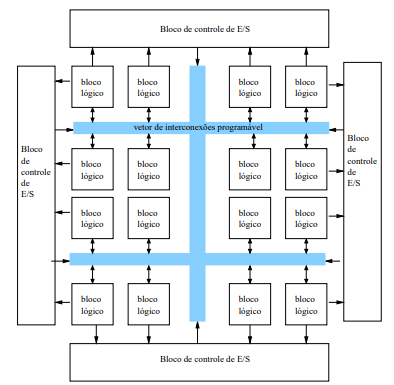
\includegraphics[width=0.4\textwidth]{figuras/CPLD.png}
	% Caption centralizada
% 	\captionsetup{justification=centering}
	% Caption e fonte 
	 \vspace{-0.2cm}
	\\\textbf{\footnotesize Fonte: Relatório Técnico no.005 de 2002, da
área de informática do DCCE \citeonline{cap-livro} }
	\label{fig:figura1}
\end{figure}
\vspace{-0.5cm}

 \newpage \subsection{\esp FPGA}

São caratecterizados especialmente por requerir de um processo especial de fabricação, dando a este um alto custo de projeto e longa implementação, quando utilizado em grandes projetos, procura-se fazer uma divisão de testes para tentar melhorar o desempenho.

 \ref{fig:figura1}. 
% Figura
\begin{figure}[ht]
	\centering	
	\caption[\hspace{0.1cm}]{Configuração interna de uma FPGA}
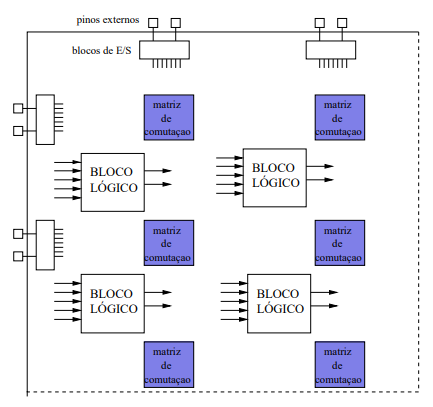
\includegraphics[width=0.4\textwidth]{figuras/FPGA.png}
	% Caption centralizada
% 	\captionsetup{justification=centering}
	% Caption e fonte 
	 \vspace{-0.2cm}
	\\\textbf{\footnotesize Fonte: Relatório Técnico no.005 de 2002, da área de informática do DCCE}
	\label{fig:figura1}
\end{figure}
\vspace{-0.5cm}

\newpage
\section{REFERÊNCIAS}
O.A.C.Macedo; P.B.Alves;  N.Marranghello. DISPOSITIVOS LÓGICOS PROGRAMÁVEIS. UNIVERSIDADE ESTADUAL PAULISTA, nov. 2002.

FREITAS, Tiago Tobias; PASQUALIANOTO, Thiago Luiz; LEÃO, Juliano Carlos Leão.1O CPLD (Dispositivo Complexo de Lógica Programação aplicado em automação industrial. Feira SENAI Paulista de Inovação Tecnológica  -  INOVASENAI, 2005.

 CODÁ, Luiza Maria Romeiro. DISPOSITIVOS LÓGICOS PROGRAMÁVEIS. Departamento de Engenharia Elétrica e de Computação.
 

 


%%%%%%%%%%%%%%%%%%%%%%%%%%%%%%%%%%%
%% FIM DO TEXTO
%%%%%%%%%%%%%%%%%%%%%%%%%%%%%%%%%%%

% \selectlanguage{brazil}
%%%%%%%%%%%%%%%%%%%%%%%%%%%%%%%%%%%
%% Inicio bibliografia
%%%%%%%%%%%%%%%%%%%%%%%%%%%%%%%%%%%



\end{document}


